% Compile with XeLaTeX twice, or: tectonic main.tex
\documentclass[UTF8,a4paper,11pt,fontset=fandol]{ctexart}
\usepackage[margin=18mm,headheight=15pt,footskip=10mm]{geometry}
\usepackage{amsmath,amssymb,graphicx,booktabs,array,pdflscape}
\usepackage{xcolor,hyperref,fancyhdr,enumitem}
\definecolor{ink}{HTML}{193D65}
\hypersetup{colorlinks=true,urlcolor=ink,linkcolor=ink,pdftitle={圆形端面多芯光纤：四方法比较},pdfauthor={}}
\pagestyle{fancy}\fancyhf{}
\fancyhead[L]{\small 圆形端面多芯光纤：四方法比较}
\fancyhead[R]{\small 2026年10月4日修订}
\fancyfoot[C]{\thepage}
\setlength{\parindent}{0pt}\setlength{\parskip}{5pt}
\setlist[itemize]{leftmargin=1.5em,itemsep=3pt,topsep=2pt}
\ctexset{section={format=\Large\bfseries\color{ink}},subsection={format=\normalsize\bfseries\color{ink}}}
\renewcommand{\arraystretch}{1.35}
\newcommand{\electron}{\mathrm{e}^{-}}
\newcommand{\figpage}[4]{%
\clearpage\begin{landscape}\thispagestyle{empty}
\section*{#1}
\begin{center}\includegraphics[width=240mm,height=135mm,keepaspectratio]{figures/#2}\end{center}
{\small\textbf{#3}\quad #4\par}
\vfill\begin{center}{\small\thepage}\end{center}\end{landscape}}
\begin{document}
\begin{center}
{\LARGE\bfseries\color{ink}圆形端面多芯光纤：四方法比较}\par
\vspace{3pt}阶段汇报\enspace |\enspace 呈佳伟老师
\end{center}
佳伟老师：本阶段完成圆形端面多芯光纤（MCF）的周期与非周期两类模拟，在统一输入、初值和传播预算下比较 HIO、ER、RAAR 与 L-BFGS。16 项求解任务全部完成，几何检查和数值测试均通过。
\subsection*{主要发现}
\begin{itemize}
\item 无噪声时，两类布局均以 RAAR 的复场误差最低。
\item 含噪声时，四种算法中 ER 的复场误差最低；但传播预算由 80 增至 200 后，误差反而上升。
\item 含噪声时，四种算法的相位误差均高于初始参考，提示需进一步检查噪声处理与停止准则。
\end{itemize}
\subsection*{核心结果：复场 NRMSE，越小越好}
\begin{center}\small
\begin{tabular}{lrrrrr}\toprule
布局 / 测量 & 初始参考 & HIO & ER & RAAR & L-BFGS\\\midrule
周期 / 无噪声 & 0.6555 & 0.1489 & 0.1475 & \textbf{0.1182} & 0.2123\\
非周期 / 无噪声 & 0.6739 & 0.1267 & 0.1292 & \textbf{0.1027} & 0.1523\\
周期 / 含噪声 & 0.6555 & 1.3988 & \textbf{0.6313} & 0.9480 & 0.8608\\
非周期 / 含噪声 & 0.6739 & 1.3830 & \textbf{0.6231} & 0.9260 & 0.8542\\\bottomrule
\end{tabular}\end{center}
四种算法均使用 200 次传播；初始参考为共同起点，未迭代。粗体表示四种算法中的最低复场误差。复场误差同时反映振幅与相位偏差，仅对齐一个全局相位；精确定义见第~\pageref{sec:metrics}~页。
\subsection*{增加计算量未改善含噪声结果}
\begin{center}
\begin{tabular}{lrr}\toprule
含噪声 ER & 80 次传播 & 200 次传播\\\midrule
周期 & 0.5487 & 0.6313\\
非周期 & 0.5495 & 0.6231\\\bottomrule
\end{tabular}\end{center}
本轮为固定种子、单个混合样品的合成试运行，采用已知参考复场；上述结论限于本轮条件。请佳伟老师指导下一阶段的工作重点。

\clearpage\section*{模型与比较条件}
\begin{center}
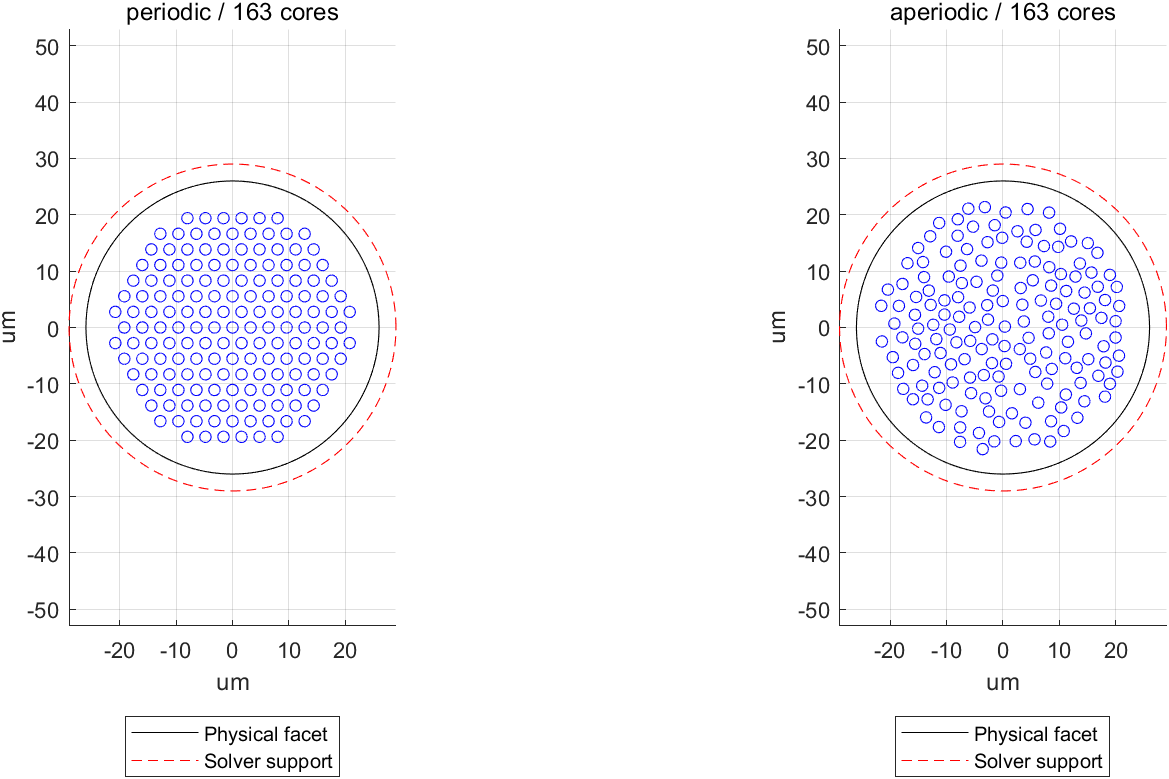
\includegraphics[width=.88\linewidth,height=93mm,keepaspectratio]{figures/geometry.png}
\end{center}
{\small\textbf{图1：实际运行布局。} 左为周期，右为非周期。黑实线为物理端面，红虚线为算法支持域，蓝圈为纤芯。两组均为 163 芯，坐标单位为 $\mu\mathrm{m}$。}
\subsection*{共同条件}
\begin{itemize}
\item 物理端面半径 $26\,\mu\mathrm{m}$，芯中心范围半径 $22\,\mu\mathrm{m}$，算法支持域半径 $29\,\mu\mathrm{m}$。
\item 周期组芯间距 $3.2\,\mu\mathrm{m}$；非周期组最小芯间距 $2.4\,\mu\mathrm{m}$。端面外场能量检查为零。
\item 两组使用同一混合样品、已知合成参考校准和共同初始化规则；四算法复用对应条件下同一保存的测量输入。
\item 计算量按传播调用次数统一计数，包含 L-BFGS 线搜索中的拒绝试探，记录 80、200 次两个预算点。参数在评分前固定。
\end{itemize}
四方法计算、评分及原始绘图共 32.62 秒，不含输入生成。此报告只重新排版和绘图，未重新运行求解器。
\subsection*{材料索引}
第~\pageref{sec:noise}~页给出噪声模型，第~\pageref{sec:metrics}~页给出实际噪声强度和误差定义；其后给出精度随迭代次数和传播次数变化的对比图，以及振幅与相位大图。
\href{https://github.com/BoVVENGibNieAuf/LSA-FAST-Phase-Retrieval-Benchmark}{公开项目仓库（无需访问授权）}保存完整代码、运行指标和结果包。本工程的 \texttt{main.tex} 与 \texttt{figures/} 可独立编译为本报告。

\clearpage\section*{噪声模型：从探测器强度到输入振幅}\label{sec:noise}
令 $I_p\ge0$ 为第 $p$ 个探测器像素的无噪声强度（细网格传播后进行像素平均），$I_{\mathrm{ref},p}$ 为空白参考帧强度。曝光换算系数定义为
\begin{equation}
\alpha=\frac{N_{\mathrm{ref}}}{\sum_p I_{\mathrm{ref},p}},
\qquad N_{\mathrm{ref}}=2\times10^5\ \electron .
\label{eq:exposure}
\end{equation}
$\alpha$ 将模拟强度换算为期望光电子数；本轮两种布局均约为 $50$。\textbf{20 万是整个空白参考帧的总期望光电子数}，不是每像素计数，也不是样品帧实际计数。未单独建模量子效率，因此不能直接解释为入射光子数。
\subsection*{散粒噪声与读出噪声}
每个像素独立生成泊松计数和零均值高斯读出噪声：
\begin{align}
\mu_p&=\alpha I_p, & K_p&\sim\operatorname{Poisson}(\mu_p),\label{eq:poisson}\\
\varepsilon_p&\sim\mathcal N(0,\sigma_r^2), &\sigma_r&=1\ \electron\quad\text{（每像素标准差）}.\label{eq:read}
\end{align}
这里 $K_p$ 以电子个数计，$\mu_p$ 是其期望值；$K_p$ 与 $\varepsilon_p$ 独立。相机读数、负值截断和输入振幅依次为
\begin{align}
Y_p&=K_p+\varepsilon_p,\label{eq:readout}\\
C_p&=\max\{Y_p,0\},\label{eq:clip}\\
A_p&=\sqrt{\frac{C_p}{\alpha}}.\label{eq:amplitude}
\end{align}
无噪声对照直接使用 $A_p^{\mathrm{clean}}=\sqrt{I_p}$。噪声施加在探测器计数层，再转换为算法输入振幅。
\subsection*{统计解释}
在负值截断\textbf{之前}，按电子计数的数值单位有
\begin{equation}
\mathbb E[Y_p]=\mu_p,\qquad
\operatorname{Var}(Y_p)=\mu_p+\sigma_r^2.
\label{eq:moments}
\end{equation}
散粒噪声随信号强度变化，不能用固定百分比概括。负值截断会在暗区引入正偏；开方后的振幅噪声也不再是加性高斯噪声。式~\eqref{eq:moments} 不适用于截断后的 $C_p$ 或开方后的 $A_p$。

\clearpage\section*{实际噪声强度与评价定义}\label{sec:metrics}
\subsection*{本轮实际计数}
探测器为 $256\times256$ 像素。空白参考帧每像素平均期望计数为 $200000/65536\approx3.052\ \electron$；样品透射损耗使总期望计数降低。
\begin{center}\small
\begin{tabular}{lrrrr}\toprule
布局 & 样品总期望电子 & 每像素均值 & 每像素峰值 & 负读数比例\\\midrule
周期 & 84114.1 & 1.283 & 68.85 & 39.19\%\\
非周期 & 82522.7 & 1.259 & 92.03 & 38.90\%\\\bottomrule
\end{tabular}\end{center}
计数由保存的无噪声强度与曝光系数计算；负读数比例取自运行记录，定义为全部 65536 个像素中 $Y_p<0$ 的比例，包含大量暗像素。

相机实现为 \texttt{fast\_mcf\_camera.m}（泊松乘积采样），MATLAB 随机生成器为 \texttt{twister}，实际种子为 3102027。两布局使用相同种子，但其 $\mu_p$ 不同，并不产生相同计数实现。每条件仅一次噪声实现，未给出跨噪声重复的置信区间。参考校准为已知合成复场，未另加校准误差。
\subsection*{误差与相位图}
令 $u$ 为恢复复场，$u_\star$ 为真值，$u_{\mathrm{ref}}$ 为已知参考复场，$\Omega$ 为保存的亮芯评分区域。全局相位对齐量为
\begin{equation}
\theta=\arg\!\left(\sum_{p\in\Omega}\overline{u_{\star,p}}\,u_p\right).
\end{equation}
复场 NRMSE 在\textbf{完整计算网格}上求范数；相位 RMSE 在 $\Omega$ 内计算：
\begin{align}
E_{\mathrm{field}}&=\frac{\lVert u\,e^{-\mathrm{i}\theta}-u_\star\rVert_2}{\lVert u_\star\rVert_2},\\
E_\phi&=\sqrt{\frac{1}{|\Omega|}\sum_{p\in\Omega}
\left[\arg\!\left(u_p\,e^{-\mathrm{i}\theta}\overline{u_{\star,p}}\right)\right]^2}.
\end{align}
相位图展示参考校正相位，定义为
\begin{equation}
\phi_p^{\mathrm{plot}}=\arg\!\left(u_p\,\overline{u_{\mathrm{ref},p}}\,e^{-\mathrm{i}\theta}\right),\qquad p\in\Omega.
\label{eq:phaseplot}
\end{equation}
$\Omega$ 为支持域内参考振幅大于参考峰值 $15\%$ 的像素。白色为未显示区域，不代表零相位；相位图与相位误差含义不同。所有相位图共用 $[-\pi,\pi]$ 色标，所有振幅图共用同一色标，未逐图归一化。

\figpage{精度随迭代次数变化｜复场误差}{convergence_field_nrmse_iterations.pdf}{图2}{复场 NRMSE 越低越好。圆点为实际保存的初值、80 次与 200 次传播检查点；连线仅辅助辨认，不表示逐步记录或插值估计。HIO、ER、RAAR 对应第 0、40、100 轮；L-BFGS 横坐标为各条件下实际接受的更新次数。四种条件分别展示，初值相同。}
\figpage{等计算预算下的精度变化｜复场误差}{convergence_field_nrmse_propagations.pdf}{图3}{横轴为正向与伴随传播的累计调用次数，包含 L-BFGS 被拒绝的线搜索试探；用于等传播预算比较。各曲线仅包含 0、80、200 三个真实检查点，连线不代表中间轨迹。含噪声 ER 从 80 到 200 次传播的复场误差上升。}
\figpage{精度随迭代次数变化｜相位误差}{convergence_phase_rmse_rad_iterations.pdf}{图4}{亮芯区域内全局相位对齐后的相位 RMSE，单位 rad，越低越好。点的位置采用实际接受的迭代次数；L-BFGS 每轮的传播开销可变。仅显示保存的三个检查点，不推断未记录区间的波动或最佳停止位置。}
\figpage{等计算预算下的精度变化｜相位误差}{convergence_phase_rmse_rad_propagations.pdf}{图5}{与图4使用同一组相位误差，改以传播次数为横轴。全部数值来自原批次指标，并与报告终值一致；本次未获得逐迭代密集记录。图中比较限于原单样品、固定种子运行，无重复实验置信区间。}
\figpage{周期 / 无噪声｜振幅比较}{periodic_clean_amplitude.pdf}{图6}{六面板为真值、共同初值、HIO、ER、RAAR、L-BFGS。四算法预算均为 200 次传播。显示范围 $\pm32\,\mu\mathrm{m}$，覆盖半径 $29\,\mu\mathrm{m}$ 的支持域；完整计算网格宽 $128\,\mu\mathrm{m}$。}
\figpage{周期 / 无噪声｜相位比较}{periodic_clean_phase.pdf}{图7}{参考校正相位见式~\eqref{eq:phaseplot}。仅显示保存的亮芯区域 $\Omega$；白色区域不代表零相位。色标统一为 $[-\pi,\pi]$，单位为 rad。算法顺序与振幅图一致。}
\figpage{非周期 / 无噪声｜振幅比较}{aperiodic_clean_amplitude.pdf}{图8}{六面板为真值、共同初值、HIO、ER、RAAR、L-BFGS。四算法预算均为 200 次传播。显示范围 $\pm32\,\mu\mathrm{m}$，覆盖半径 $29\,\mu\mathrm{m}$ 的支持域；完整计算网格宽 $128\,\mu\mathrm{m}$。}
\figpage{非周期 / 无噪声｜相位比较}{aperiodic_clean_phase.pdf}{图9}{参考校正相位见式~\eqref{eq:phaseplot}。仅显示保存的亮芯区域 $\Omega$；白色区域不代表零相位。色标统一为 $[-\pi,\pi]$，单位为 rad。算法顺序与振幅图一致。}
\figpage{周期 / 含噪声｜振幅比较}{periodic_shot_read_amplitude.pdf}{图10}{六面板为真值、共同初值、HIO、ER、RAAR、L-BFGS。四算法预算均为 200 次传播。显示范围 $\pm32\,\mu\mathrm{m}$，覆盖半径 $29\,\mu\mathrm{m}$ 的支持域；完整计算网格宽 $128\,\mu\mathrm{m}$。}
\figpage{周期 / 含噪声｜相位比较}{periodic_shot_read_phase.pdf}{图11}{参考校正相位见式~\eqref{eq:phaseplot}。仅显示保存的亮芯区域 $\Omega$；白色区域不代表零相位。色标统一为 $[-\pi,\pi]$，单位为 rad。算法顺序与振幅图一致。}
\figpage{非周期 / 含噪声｜振幅比较}{aperiodic_shot_read_amplitude.pdf}{图12}{六面板为真值、共同初值、HIO、ER、RAAR、L-BFGS。四算法预算均为 200 次传播。显示范围 $\pm32\,\mu\mathrm{m}$，覆盖半径 $29\,\mu\mathrm{m}$ 的支持域；完整计算网格宽 $128\,\mu\mathrm{m}$。}
\figpage{非周期 / 含噪声｜相位比较}{aperiodic_shot_read_phase.pdf}{图13}{参考校正相位见式~\eqref{eq:phaseplot}。仅显示保存的亮芯区域 $\Omega$；白色区域不代表零相位。色标统一为 $[-\pi,\pi]$，单位为 rad。算法顺序与振幅图一致。}
\end{document}
